\section{Approaches}\label{Approaches}
    In this section, the more detailed information about approaches can be used in the development of our proposed will be explained. For one task, there might be more than one approaches with different advantages and disadvantages, the decision on using which approaches should be done with consideration of resources. The analyzation toward approaches will be shown as same order in section \ref{problem}, which is data, model and software.
        \subsection{Data}
            \subsubsection{Data collection}
                %Add specific data found. ADD ABOUT TEXT DATA
                The data collection work would focus on taking relatively reliable data from internet with as high quality and quantity as possible. 

                There are major two ways in collecting data online, one is use dataset made by other researchers or companies, another way is collecting data from internet through web scraping by ourselves.

                Considered that the amount of data of eczema is generally insufficient, we would need data integration, which combine different data from different channel together to form a larger dataset.

                For using of exist dataset, there are multiple famous websites that share dataset made by others. Here are some typical sources:
                \begin{enumerate}
                    \item Kaggle, a famous data science competition platform with a large amount of dataset resources done by other data scientists.
                    \item Paper With Code, a famous platform that store code used in papers, also include dataset resources used in researches.
                    \item Google dataset search, a search engine that provide searching service among internet for usable datasets.
                    \item Conference / company machine learning competition, some competitions held by academic conferences or companies will give out dataset resources.
                \end{enumerate}

                From above sources, we can find some dermatological datasets that might be useful in our model. For eczema dataset, the quality is not satisfying since there are so much background noises and the quantity is not enough. However, it's still better than nothing. Collecting more data from other channel thus became more important and necessary. For general dermatology data, some well-known dataset like ISIC and HAM10000\cite{DVN/DBW86T_2018}

                For the second way, collecting data from internet through web scraping. It is possible to scrap images from websites like Google Image automatically through scripts. There are various libraries that support automatic data scraping with a few lines of code, for instance, Selenium and Beautiful Soup in python are popular libraries that help scraping data from websites. However, the data scraped from internet generally have a low quality as well, so manual cleaning would be necessary after collecting these data. Furthermore, the data scraped from websites may not be accurate, and the lack of examination from professional dermatologists may cause wrong data in dataset. Therefore, the use of web scraped data should be careful.

                Furthermore, there is another way to collect data, which is using generative models to generate data. However, the generated medical data may not be accurate enough, so this method should be used with extra careness.

                In addition, since we might need natural language processing(NLP) models for our suggestion model, we might need text data. Fortunately, the collection of text data is much easier than image data due to its large volume. However, since we are making models for medical platform, the reliability of the data is the main concern. We would need external assistance on verifying the data. Furthermore, collecting medical text data may not be easy.

                As another part of our platform, a knowledge base on eczema relevant information is also needed, like treatment, cautions and basic information. The reliability of this knowledge base is important, the data should come from reliable and trustable sources.

                The data would be divided into three, training dataset, validation dataset and test dataset. Training dataset should take the most proportion, which is used to train the model, usually take up to 80\% of the dataset; validation dataset is for validate the performance of data during optimization and training, models will be tuned based on the result get on validation dataset, it usually takes the rest 20-40\% of the dataset; test dataset is a little different, it does not appear in the dataset during training, the test dataset is only used as the last evaluation of the model to reveal the real performance of model, theoretically, models should not be tuned on test dataset, the real cases model faced in application are also a kind of test data.

            \subsubsection{Data augmentation}\label{dataArg}
                As the following step after data collection, data augmentation aims to  improve the quality and quantity of data, solve the problems in dataset.

                The first step involves in data augmentation is data cleaning, this step focus on clean the wrong data in dataset. For instance, in one eczema dataset we found on Kaggle, there are images of dermoscopy in it, which is definitely inappropriate to train a model used to classify eczema by digital image of affection area input. These kinds of noise in dataset need to be clean in data cleaning stage of data augmentation. In addition, there might be some mistake in labelling that can be easily found out, for example, typo in class name.

                The next step of data augmentation is normalization, which focus on scaling the features of data into a same scale. This usually happened in numerical or text data since multiple features of same thing would be shown in dataset. For instance, in predicting house price, the area of house and the listing price are in totally different scale, the model would ignore the area data since the price are much larger than the area. Normalization of data can prevent it by rescale the data into one. However, since we are mainly working on image data, normalization of data is not that important, but we may still need to scale the RGB value of images into 0-1 instead of 0-255 for better computational performance.

                Next step of data augmentation is transformation, which mainly happened in image data to form a larger and more diverse dataset. The main idea is to use various method to transform the image data into another image, thus increase the size of dataset and the generalizability of model through creating data that happened under more scenarios. For instance, transform the brightness of image data can simulate the situation of taking picture under different light conditions, flipping images can simulate taking picture in other angles. Through training more diverse data, the generalizability of model can increase. 

                There are several methods for transformational augmentation of image data, usually people will use multiple method at same time to improve the dataset. Common image data augmentation methods are:
                \begin{enumerate}
                    \item Flipping, through random flipping the image into other direction to create new image data that increase the size the dataset.
                    \item Rotation, through rotating the image into random angles to make the dataset more diverse and larger.
                    \item Random Crop, cut certain area of image data at random position to form new image data to simulate the scenarios of users taking incomplete pictures as input while increasing the dataset size.
                    \item Mix up, random crop images and concatenate them into one picture, can help reduce overfitting and improve model performance.
                    \item Brightness change, randomly change brightness of image data to simulate scenarios under different light conditions while making the dataset larger.
                    \item Saturation change, randomly change the saturation of image, to simulate different scenarios while expanding the dataset.
                    \item Hue change, randomly change the hue of data to simulate scenarios and increase the dataset size.
                \end{enumerate}

                Among above methods, some operations involve change of color may not be appropriate in our case since the color of input picture could be important in identification of skin disease. Choosing augmentation methods would need experiments on the effect and result.
                
                Usually, transformation of data would be conducted together with training of model as a part of the networks. Technically, the implement of common transformation method has been done by the machine learning framework, so the implement would not the problem, design of transformation method used is the main focus in this part.

                Since the scarcity of some eczema subtypes, the collection of equal amount of all eczema subtypes are difficult. Therefore, we would need methods to solve the imbalanced class distribution in dataset. To solve the problem, we need resampling.

                There are generally two method of resampling, cross-validation and bootstrap. Basically these techniques balance the data during training by sampling the class that with insufficient data more during the training process. Fortunately, the implementation of these techniques has been done by frameworks, although the implement from sketch is not challenging either.

                Apart from augmentation on the actual data in dataset, another possible process toward data would be labeling. Although the image data are usually labelled into class already, we might need to label data if we need more information on data, like position. Considered we might need object detection algorithm, we would need the label the bounding boxes of affected area. There are multiple approaches, the easiest one is simply labeling the data manually, there are plentiful software that can help with drawing bounding box on data, the manual operation can ensure the quality of labeling as well, but manual labeling of data would result in high labeling cost as well. Another method is half-automatic labeling by using pre-trained object detection models and manual checking, this method can save human resources on labeling while ensuring quality, but it would require a high quality pre-trained model that fit well in medical tasks. There is several software programs developed with pre-trained models that allow users to label with aid of AI.
                %FEATURE ENGINEERING
        \subsection{Model}

            Model is the key part of our research, and the most expensive part. To reduce the training cost, one common method is transfer learning or fine-tuning, which use pre-trained model in other datasets as base to fit into our desire problem.

            \subsubsection{Model design}
                \paragraph{Diagnosis model:}
                    The diagnosis model is the model that provide the initial diagnosis of eczema, basically whether the users have eczema or not with input about their skin. There are multiple approaches toward this model.

                    For our diagnosis model, there are two possible inputs, image input of affected area, or a text input in either a survey or natural language form. Both input methods are possible for our platform but with different advantages and disadvantages.

                    Firstly, image input, using image input mean we need to design a model that can diagnosis eczema from digital images of affected area, which can be seen as an image binary classification problem that have two classes, eczema class and a negative class.

                    Since it is a classification model that have similar solution stack with our proposed classification model used in classify eczema subtypes. Detailed of model choices would be explained in next paragraph that mainly focus on classification model. Generally, image classification models would need large amount of labeled data on both eczema image and non-eczema image. Considered there are various skin disease that have similar appearances to eczema, data of similar disease would also be needed as negative class.

                    For text input, there are more possible approaches. Firstly, the input of text can be in different forms, the easiest form would be a survey form, by pre-defined a survey covered relevant question about eczema, or a more complex but user-friendly method is using natural language input that allows the users using natural language to describe their situation.

                    To achieve a natural language input, we would need natural language process model(NLP). NLP models can process natural language by using deep learning algorithms, the most common one nowadays would be transformer. From chatGPT to Deepseek, the introduction of transformer is one of the most important progress in deep learning over the past decade. Transformer is an architecture that use attention mechanisms(will be explained detailedly later in the paper) that designed for processing natural text.
                    \begin{Figure}
                        \centering
                        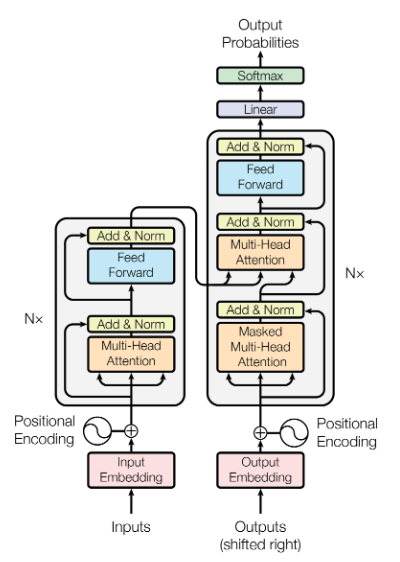
\includegraphics[width=\linewidth]{Image/Transformer.png}
                        \captionof{figure}{Architecture of transformer model\cite{vaswani2017attention}}
                    \end{Figure}

                    With NLP, not only the natural input is possible, outputs in natural language is also possible. The application of NLP in natural output would be further discussed in section \ref{suggestion}.

                    However, training a NLP from sketch is impossible since it required massive amount of data and training resources. Therefore, the approach toward NLP would be fine-tuning on pre-trained transformer. Before introducing the transformer we used, we need to understand an architecture first. Encoder-decoder architecture is a powerful architecture that have been proven to be useful in multiple aspects, the main idea of encoder-decoder architecture is separating the model into two parts, encoder and decoder, where encoder are part that convert the input into highly abstract features, and decoder are part that convert these highly abstract features into outputs. BERT\cite{devlin2019bert}, is a bidirectional transformer encoder that was pre-trained on massive of text data. By adding decoder on top of BERT, state-of-art models can be created by fine-tuning. This allows application of NLP in different aspect easily, in our case, we can create a model that take the user's description as input, the initial diagnosis result as output. The major barrier on this design would be data, this application of data would require text dataset that include users' description and diagnosis result, which can be hard to collect.

                    The advantages for image classification approach are the relatively lower difficulty in data collection and lower training cost, but the disadvantages would be less intuitive user experience, and less information collected from users for the later suggestion model. For NLP approach, the main advantages are more intuitive user experience and a more comprehensive diagnosis based on users' description, but with the disadvantages include higher data collection difficulty and higher training cost.

                    Furthermore, image can also be taken as the input while using text as input to provide a more comprehensive prediction. Therefore, it's possible to combine both image classification model and NLP to build our diagnosis model.
                \paragraph{Classification model:}
                    The classification model in our platform play the most vital role. The classification model between different eczema type is the main feature in our platform. There are many approaches to build such a model as well. 

                    Unlike the diagnosis model may have different kind of input methods, the input of classification model is fixed as digital images in design of the platform. Therefore, the classification model is also an image recognition model. A popular approaches in image classification model is convolutional neural networks(CNNs)

                    Convolutional neural networks is a deep learning algorithm based on multi layer perceptions(MLP) models that use several convolution kernels to extract features of input, which is usually images.

                    Convolution operations in CNNs are cross correlations that sum the neighbor elements of values with certain weight in a kernel. The mathematic formula for convolution operations is\cite{zhang2023dive}:
                    \[
                        (f * g)(i, j) = \sum_a\sum_b f(a, b) g(i-a, j-b)
                    \]
                    \textit{Where the symbol $*$ mean convolution, $f, g: \mathbb{R}^d \to \mathbb{R}$ }

                    To visualize this operation, the following figure show the process of convolution in image processing.
                    \begin{Figure}
                        \centering
                        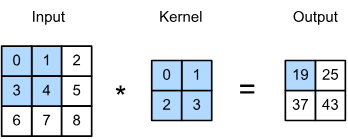
\includegraphics[width=0.8\linewidth]{Image/Conv.png}
                        \captionof{figure}{Visualized processed of convolution operation\cite{zhang2023dive}}
                    \end{Figure}

                    Convolution kernels are neurons that processed convolution operation to its input, which is the weight matrices in convolution operations, and take the result into activation function, which add nonlinearity to the model, as the output. The magnitude of convolution kernels is learnable parameters of models. The operation can be conducted into multiple channels so that more features can be extracted in a layer of network. Usually the output of convolution layers would be feed into several fully connected layers and finally get into a softmax classification layer(Not necessary, some models like NiN use $1\times1$ convolution layers to act as fully connected layers).

                    \begin{Figure}
                        \centering
                        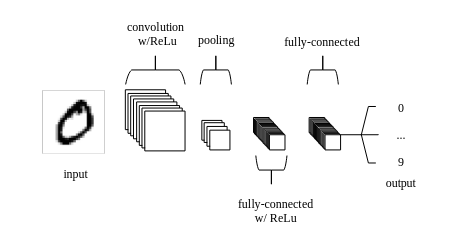
\includegraphics[width=\linewidth]{Image/CNNs.png}
                        \captionof{figure}{A simple CNNs architecture that used to recognize handwrite numbers in MNIST dataset\cite{o2015introduction}}.
                    \end{Figure}

                    The advantages of using convolution operation is that it consist with two principles in doing image processing, translation invariance and locality. The former reveal the fact that the translation of object's position does not matter in image recognition, for instance, target object present in up-right corner is same as presenting in up-left corner, so the convolutional kernel does not change with the detection position\cite{zhang2023dive}. For the latter, locality states that when recognizing image, the model should focus more on part of the image only, so the convolution operation only consist part of input at one time, which is the size of the kernel.

                    With these basic knowledge of convolutional neural networks, data scientists have designed plentiful architectures that use different method to achieve better result. Therefore, for our classification model, we would not need to design a completely new model from sketch.

                    \begin{Figure}
                        \centering
                        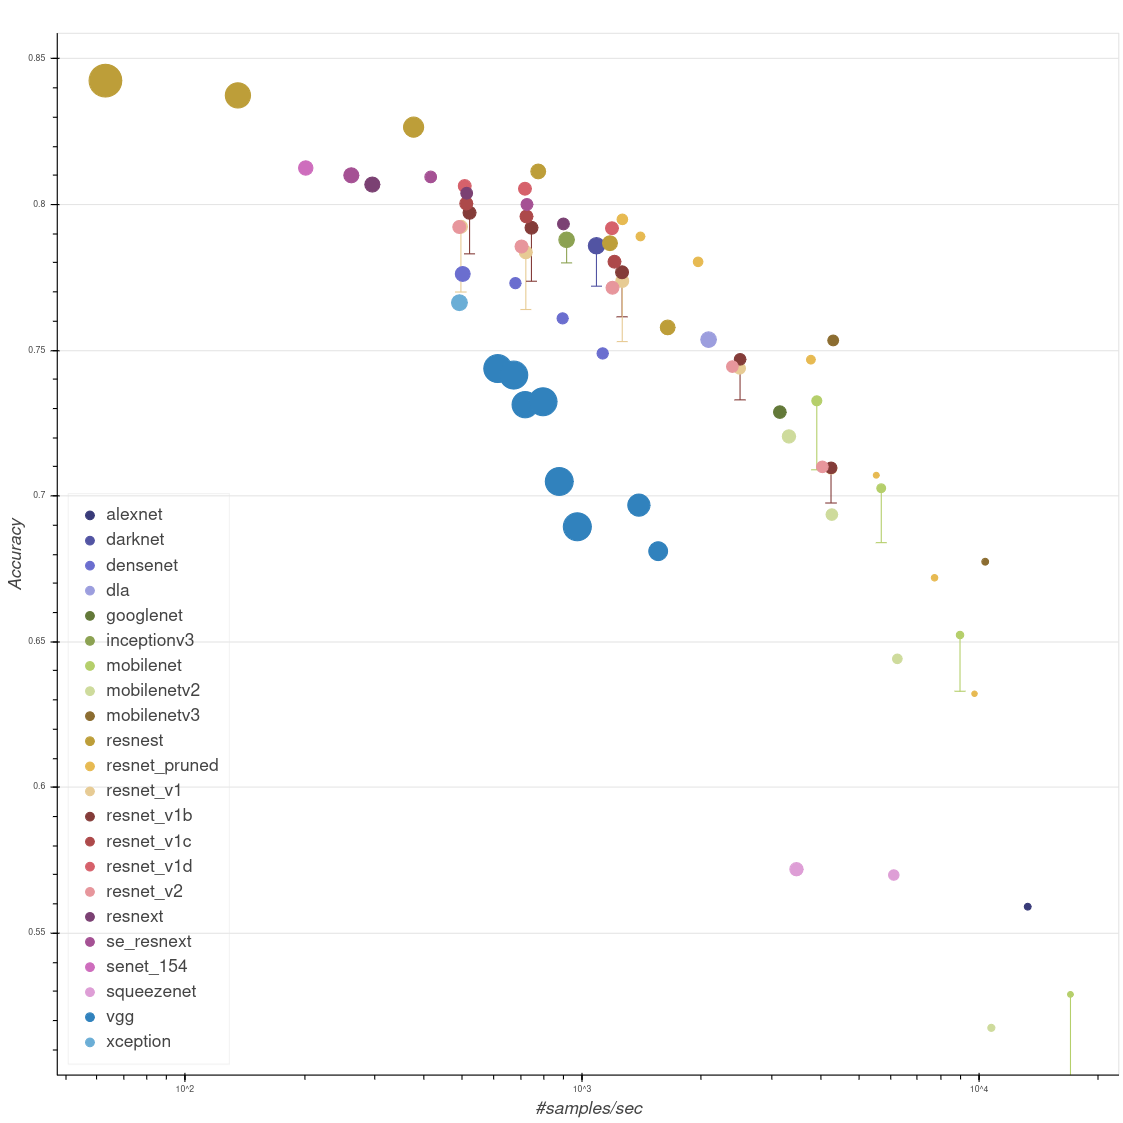
\includegraphics[width=\linewidth]{Image/bokeh_plot.png}
                        \captionof{figure}{Plot graph of some existing models, where x-axis shows respond speed, y-axis shows accuracy, the size of circle shows the size of model\cite{gluonmodel}.}
                    \end{Figure}

                    Inception V3, is a CNN model that factorized the convolution process into smaller convolution\cite{szegedy2015rethinkinginceptionarchitecturecomputer}. It used inception blocks, convolution layers and fully connected layers to create the network. The model has outstanding performance, which make it possible to be our base model.

                    \begin{Figure}
                        \centering
                        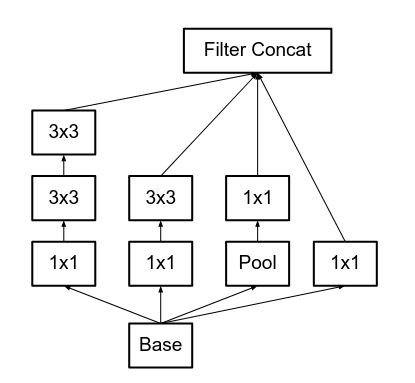
\includegraphics[width=\linewidth]{Image/Inceptiion.png}
                        \captionof{figure}{An example inception unit\cite{szegedy2015rethinkinginceptionarchitecturecomputer}}
                    \end{Figure}

                    Another model is ResNet, residual network, the main idea of ResNet is using residual learning, which add the input of a block into the output. The idea of residual learning allows training of even deeper networks and solves degradation problem that models become saturated\cite{he2015deepresiduallearningimage}. ResNet model has achieved significant result in computer vision, and has been the most popular model used.

                    \begin{Figure}
                        \centering
                        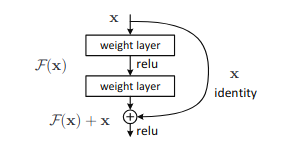
\includegraphics[width=\linewidth]{Image/Residual.png}
                        \captionof{figure}{Residual learning\cite{he2015deepresiduallearningimage}}
                    \end{Figure}

                    Although there are other machine learning algorithms can do image classification as well, like random forest, there is no significant advantages for doing so. Therefore, we choose to use deep learning algorithm as the general pathway toward our classification model.

                    With well-developed model structures, we might not need to design our own model architecture. However, if the performance on these tradition models is unsatisfying, we can design our own model architecture as well.

                    Fine-tuning, or transfer learning, is training model base on pre-trained model's parameters by adding output layers on top of the base model. Fine-tuning can largely reduce the training cost and the amount of data needed. Usually, the result of transfer learning would be better if the base model are trained for similar problem on similar datasets. In academia, the common dataset used is ImageNet\cite{imagenet_cvpr09}, a large scale image dataset for computer vision competitions consist objects can be seen in daily life. The problem is, using pre-trained models that trained on ImageNet may not be suitable for a dermatology classification task. Therefore, we might consider pre-training models on dermatology dataset like ISIC and HAM10000. Notice that transfer learning does not necessarily mean using others' model design, it is possible to create our own model architectures and pre-train it on larger dataset to reduce the amount of data needed.
                    
                    There is another challenging part in classification work that the input picture, both in dataset and actual usage, may not be taken perfectly without background noises. Therefore, how to make the model not to be disturbed by the background noises is important.

                    A simple method toward it is using object detection algorithm to aim the affection area only. Unlike basic image classification model that can be designed and made by ourselves, although the implement an object detection model from its underlying theory may not be very difficult, a developed algorithm still take times for optimization, so there is no point for reinventing the wheel.

                    There are plentiful options for object detection, a common approach is using CNNs to predict the position of bounding box in image.
                    
                    R-CNN\cite{girshick2014rich}, region-based CNNs, is a classic object detection model. Generally, it used selective search to get region proposals like anchor boxes in image, and follow with CNNs or support vector machines(another machine learning algorithm) to predict the classes and positions of bounding boxes\cite{uijlings2013selective}. There is a series of model based on the idea of R-CNN, including fast R-CNN\cite{girshick2015fast}, faster R-CNN\cite{ren2015faster} and mask R-CNN\cite{he2017mask} that improve the architecture to get better accuracy or efficiency.
                    \begin{Figure}
                        \centering
                        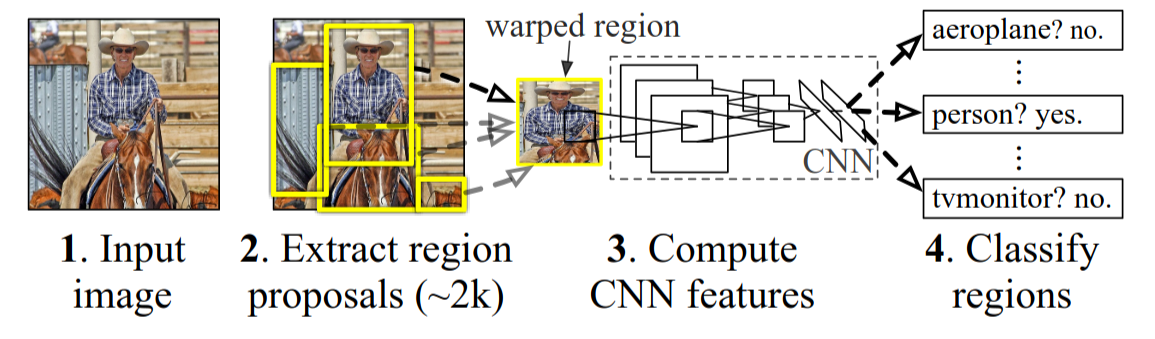
\includegraphics[width=\linewidth]{Image/R-CNN.png}
                        \captionof{figure}{R-CNN overview\cite{girshick2014rich}}
                    \end{Figure}

                    Another classic object detection algorithm is SSD, single shot multibox detection\cite{liu2016ssd}, the model using anchor boxes that extracted from feature maps(the output of convolution layers) and predict classes and positions using CNNs. YOLO, you only look once, improve the model by separating the image in the different pieces to reduce the overlapping of anchor boxes, thus achieved a higher speed\cite{redmon2016you}. The YOLO model is further developed, there are a lot of YOLO-based models that gain significant improvement. 

                    \begin{Figure}
                        \centering
                        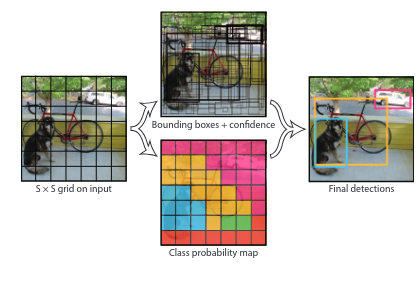
\includegraphics[width=\linewidth]{Image/YOLO.png}
                        \captionof{figure}{Idea of YOLO models\cite{redmon2016you}}
                    \end{Figure}
                    
                    Object detection models like SSD and YOLO are called one stage models compare to the two stage models like R-CNN based models since it omit the stage that search for region proposals. The change resulted in a much faster responding speed in one stage models compare to two stage models, but also lead to less accuracy due to the imbalance of negative sample(background) and positive samples.

                    In our case, we required a high accuracy model, and the responding speed of model might not be that important since the platform does not require real-time detections. However, the efficiency of the model could be important for deployment on edges. Therefore, both R-CNN based model and YOLO series are possible for us.
                    
                    A disadvantage of using object detection models are the requirement in data. Above supervised object detection algorithm required extra labelling in dataset, which is the bounding box. This will require extra work on labelling the data. There are some different way toward labelling bounding box, which can refer to the prior section \ref{dataArg}.

                    Another method to eliminate the effect of background noises is by changing the CNN model design to make it focus on specific area more.

                    Attention mechanisms are originated form NLP, but has been adapted to computer vision tasks to improve the performance of models on spatial data. The mechanisms originally used for text translation to help to memorize long source sentence\cite{bahdanau2014neural}. As the most exciting concepts introduced in deep learning in the past decade, the attention mechanisms aim to focus on related features, it takes idea from psychology that people will put their attention on the related item, for instance, if a person on street wants to read books, the person will focus on book stores or libraries they see. The three main concepts in attention mechanisms is queries, keys and values. The queries are the hints that indicate what to focus, which is "read books" in the previous example; keys and values are pairs in data, which values are the actual inputs, like "book stores" and "libraries" as an input from eyes, keys are used to pointing these values; returning a value can be done by comparing the keys and queries. What attention mechanisms do is focus on needed features by returning values based on queries. The formula of the mechanisms can be shown as:
                    \[
                        Attention(q)=\sum_{i=1}^{m}\alpha(q_i,k_i)v_i
                    \]
                    \textit{Where q is the queries, $\alpha(q,k)$ is the attention score function that calculate the similarity between query and key v is the values}

                    The attention score in the formula is a function used to determine the similarity of keys and queries. There various attention score functions, in deep learning, there will be a learnable parameter in the score function for machine learning.

                    Based on the basic idea of attention mechanisms, there are more technique developed from it. For instance, self-attention\cite{cheng2016long} is an attention that take its input as queries, keys and values at the same time, the design allows attention mechanisms to locate the related position of input. Multi-head attention is another algorithm, it takes several attention pooling on a same input to allow the model jointly attend to information from different subspaces at different position\cite{vaswani2017attention}.

                    In computer vision, there are various application of attention mechanisms, including channel attention and spatial attention, former use attention mechanisms to allow model focus on the most relevant channel(color or texture), latter use attention to allow model focus on certain relevant area on image. Both of them can be used in our model for eczema related classification. 

                    CBAM, convolutional block attention module, is an example of application of attention mechanisms in convolutional neural networks\cite{woo2018cbam}. The module proposed a convolution module using attention on both channel and spatial dimension to make the model focus on the relevant area of image. The module has shown consistently result in improving the performance of models.

                    For the classification task in diagnosis model, it is generally similar to classification between subtypes. We could place several skin diseases that have similar appearance with eczema as negative classes, together with health skin data to create the dataset. Then use similar image classification solutions to build the diagnosis model.

                    In conclusion, the three approaches toward image classification model are: CNNs, object detection models and CNNs with attention. The main advantages of CNNs are the relatively lower complexity and training cost, but the disadvantages are the risk being affected by background noises. For object detection models, the advantages are a more accuracy classification without background noises, and extra position information provided to users, the disadvantages are the need of labelling data. The advantages of CNNs with attention are robustness toward background noises without the need of extra data labelling, the disadvantages are potential higher training cost and complexity. Overall, all three approaches can be used for image classification work, however, CNNs with attention and object detection models might be better while the final decision should be made with support of practical evidence from experiments.
                \paragraph{Suggestion model:} \label{suggestion}
                    The purpose of suggestion model is provide personalized information to users after using the above models to have initial diagnosis and eczema subtypes. There are many data input the model can leverage, including the text input from users in diagnosis model, survey result, eczema subtype and image of affected area. Based on the input, the model should output the relevant information or advice about eczema, like the treatment method and self-care recommendation. The model would need to lie on a comprehensive knowledge base includes information about eczema. For instance, if the model receive input of atopic dermatitis it should return information about atopic dermatitis, and the cautions in daily life. There are multiple approaches toward this problem as well.

                    The suggestion model can be done easily, even without any machine learning technology involved. By creating pre-defined information for different subtypes and merely search for the relevant one and send out as output. This approach is extremely easy since it just sends out the pre-defined information out based on the subtype information. However, this approach also get the minimum personalized and there is no difference between users checking Wikipedia themselves. Therefore, solely using this approach is unacceptable.

                    To be a bit more advance, instead of just send out pre-defined information based on the subtype information, we can have more pre-defined information based on other users' input. For instance, using the age of users to provide more personal advice that considered the self-care measurement differences between ages. Although this approach is more personalized than the prior one, the essence of the system is still sending out pre-defined information, which is still not actual personalized advice since it is impossible to cover all the possible cases of users' input. For example, the input of users' description of itchiness would not be used if it is in text. In addition, this method would need massive workload on writing these pre-defined advices. Therefore, this approach may not be the best solution as well.

                    As a solution toward above question, we would need some machine learning algorithm to make the system or model more personalized for users. NLP would be the solution. The use of NLP allows process toward complex user inputs, like a description, this allows suggestion based on more intuitive input and ultimately personalized advices. To implement it, we would need to fine-tune pre-trained transformer(a collection attention mechanisms and neural networks originally used for NLP models) with dermatology related text datasets. However, the use of NLP is not perfect, technically, the accuracy and robustness of NLP models is a big concern as the information generated by models may not be accurate, while these qualities is crucial in such a medical related platform. Therefore, the output of NLP models can only be treated as invalided information. Then the importance of pre-defined validated information raised. On the other hand, using NLP models would require much more data and training cost, it would need extra resources for the model training.

                    In conclusion, toward the suggestion model, there are generally two approaches, pre-defined outputs and NLP. From the side of users' experience, NLP can provide ultimate personalized information, but with concern in accuracy and robustness. Pre-defined outputs are validated, but the personalization is insufficient. Therefore, the final approach for the suggestion model might be a combination of both two approaches, with a general guide pre-defined and a more personalized output just for reference. Such approach can ensure the personalization experience while providing correct information.
            \subsubsection{Model training}
                    Model training is the process model learn parameters from datasets through optimizing the loss function. It is the cornerstone of machine learning as all parameters are optimized during the process for performing tasks like classification. For computationally intense tasks like deep learning image classification and natural language processing, training on single GPU is insufficient, therefore the technique of distributed training is crucial.

                    Distributed training is distributing the training work on multiple computation units(GPUs or severs), which called workers in distributed training. There are server ways for distributed training paralleling the training process. One way is data parallel, it split the dataset into smaller chunks, the gradient calculated for gradient descent are aggregated together across different worker for parameters update. Model parallel is another way, which instead of split the dataset, it split the model into chunks, each worker account of a proportion of computation to cope with too large model that the memory of a single computational device can not handle, it would need careful management of workers communication. Another way is pipeline parallel, which the training was separated into sequential stages that each worker would compute different stages, especially used in training of very deep models.

                    Above the methods of distributed training, data parallel is the most suitable one in our case, since we are neither training a very large model nor a very deep one, the reason why we use distributed training is for better training performance and maximum use of resources. In addition, the implementation of data parallel is the most straightforward one, and it is the most common used in industry as well.

                    \begin{Figure}
                        \centering
                        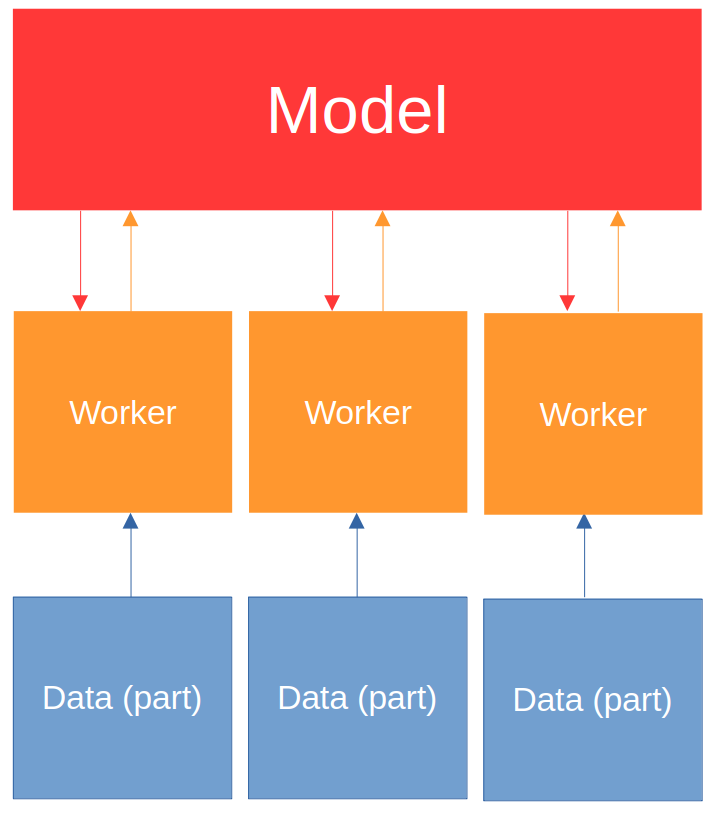
\includegraphics[width=0.9\linewidth]{Image/DataPara.png}
                        \captionof{figure}{The process of data parallels distributed training}
                    \end{Figure}

                    In distributed training, the communication between workers are the major challenge, since it is significantly slower than the communication between GPUs or memories. Therefore, the implementation of distributed training would minimize the need of communication between workers.

                    The implement of distributed in software does not need extra wariness since the related deep learning framework like TensorFlow has developed interface that can be used directly.

                    However, the implement of distributed in physical setup of server does need extra works. The setup involves the building of clusters and severs for distributed training, which need to cope with hardware and networks building.

                    Apart from distributed training, hyperparameter optimization(HPO) would be involved in model training as well. The main idea of hyperparameter optimization work is trying different parameter plan to find out the one with the best performance. The common methods include, grid search, random search and Bayesian optimization. Grid search is simply searching for every possible hyperparameters, which is very computational inefficient. Random search is search for random hyperparameters for certain rounds. Bayesian optimization is similar to random search but with statistical technique when choosing the hyperparameters. In our case, random search or Bayesian optimization would be enough.
            \subsubsection{Model evaluation}
                    As the last part of model stage, model evaluation will involve quantitative assessment toward our model. Model evaluation would involve metrics for evaluating the models' performance, choosing a correct metric would be the key part of model evaluation. The adaption of metrics would variate with the specific task model confront with, which in our case, are mainly classification.

                    In binary classification task, like our initial diagnosis(eczema or not), the main performance of model we care about is the ability of model to correctly classify the input. There are several possible outcomes, true positive(TP), true negative(TN), false positive(FP) and false negative(FN). The most common metrics toward such a binary classification task are accuracy, specificity, sensitivity and precision\cite{rainio2024evaluation}, which can be calculated by the formulas:
                    \begin{gather*}
                        Acc. = \frac{TP+TF}{TP+FP+TN+TF} \in [0,1] \\
                        Sen. = \frac{TP}{TP+FN} \in [0,1]\\
                        Spe. = \frac{TN}{TN+FP} \in [0,1]\\
                        Pre. = \frac{TP}{TP+FP} \in [0,1]
                    \end{gather*}
                    All above metrics are in the range of 0 to 1, and larger magnitude represent better performance. Among them, accuracy means the proportion of correct classification to all input, sensitivity means the proportion of correctly classified positive to number of all positive input, specificity means the proportion of correctly classified negative to number of all negative input, precision means the proportion of correctly classified positive to positive output. The sensitivity and specificity metrics can reveal more about the models' performance when the positive samples and negative samples are very imbalanced. 

                    With the above metrics, more complex metrics can be calculated, F1-score are defined as:
                    \[
                        F1 = \frac{2\cdot Pre. \cdot Sen.}{Sen. + Pre.}
                    \]
                    which is the harmonic mean of sensitivity and precision.

                    The metrics of multi-classes classification is similar but a bit more complex. Where a confusion $k\times k$ matrix of $k$ classes is built, and the values like true positive would be a macro-averaing across all classes. Then the calculation of above metrics is similar.
        \subsection{Software}
            After building up the models for our platform, here comes to the next stage of building the platform software. The building of platform can be separated into three stages as well, deployment, development and UI/UX design. 
            \subsubsection{Deployment}

            The deployment of model is important for the development of platform. The main tasks in deployment are ensuring the capability of models under certain environment, like mobile-end, and optimizing the model for better efficiency performance. Since we are working on a medical project developing a cross-platform eczema diagnosis platform, the latency, resources constraints and consistency across devices are critical.

                The model deployment work mainly consists two part, model compression for better efficiency and capability under edge environments and putting the model into the software.

                The first step in model deployment is model compression, by using different optimization algorithms to minimize the model size and increase the efficiency of model. There are three main methods toward model compression, quantization, pruning and knowledge distillation.

                Quantization optimization is the process convert the format of parameters in model from data structure like FP32 that occupied large memories to other data structure like INT8 that occupied fewer memories. There are multiple ways to do that, dynamic range quantization is only changing weights from FP32 to INT 8 while the activations value still keep as float, this optimization can reduce the model size about 75\% while have less than 1\% loss in accuracy.  Full integer quantization is converting all float value to integer, it minimized the model size but may result in larger accuracy loss.
                
                Pruning optimization reduce the computational complexity by removing the excesses neurons that have low impact toward the result. The optimization process can not only reduce the size of model, but also reduce the computational complexity since it remove unnecessary computational unit in the network.

                Knowledge distillation\cite{hinton2015distilling} is a bit more complicated, basically it transfers the knowledge of teacher model, which is the one relatively larger, to student model, which is the light model. By training a large model first and guide the training of small model with large model, knowledge distillation model can largely reduce the model size and computational complexity.

                All above methods can be used in our platform. By using these model compression methods, the model can be reduced into a size that can be run under mobile environments like Android or iOS.

                The implementation of these optimization techniques is not a problem since the deep learning frameworks has implemented relevant optimization algorithm already. For example, TensorFlow Lite allows model trained on TensorFlow convert to TensorFlow Lite models that is smaller with optimization algorithms, which is in .tflite format. With this framework, the model can be easily deployed into the software, which will be more detailed explained in section \ref{development}.
            \subsubsection{Development}\label{development}
                The development of the software is another crucial part. The main challenge in this part is building a cross-platform software, which mainly include Android and iOS, possibly Windows or web.

                Traditionally, building a multi-platform application will require developing multiple distribution version, which would need massive code and resources. Fortunately, there are frameworks that provide cross-platform development with only developing one version. One example would be Flutter

                Flutter is an open-source UI software development kit developed by Google. It can be used to develop cross-platform applications from single codebase for platforms including Web, Windows, macOS, iOS, Linux and Android. Flutter allows developer build multi-platform application without working on adaption for every platform. The architecture of Flutter involve different layers, while the developers would only need to work on the top layer on developing the application, lower lever rendering and platform specific adaption has been done by the framework. This allows cross-platform application run with high performance at the same time.

                \begin{Figure}
                    \centering
                    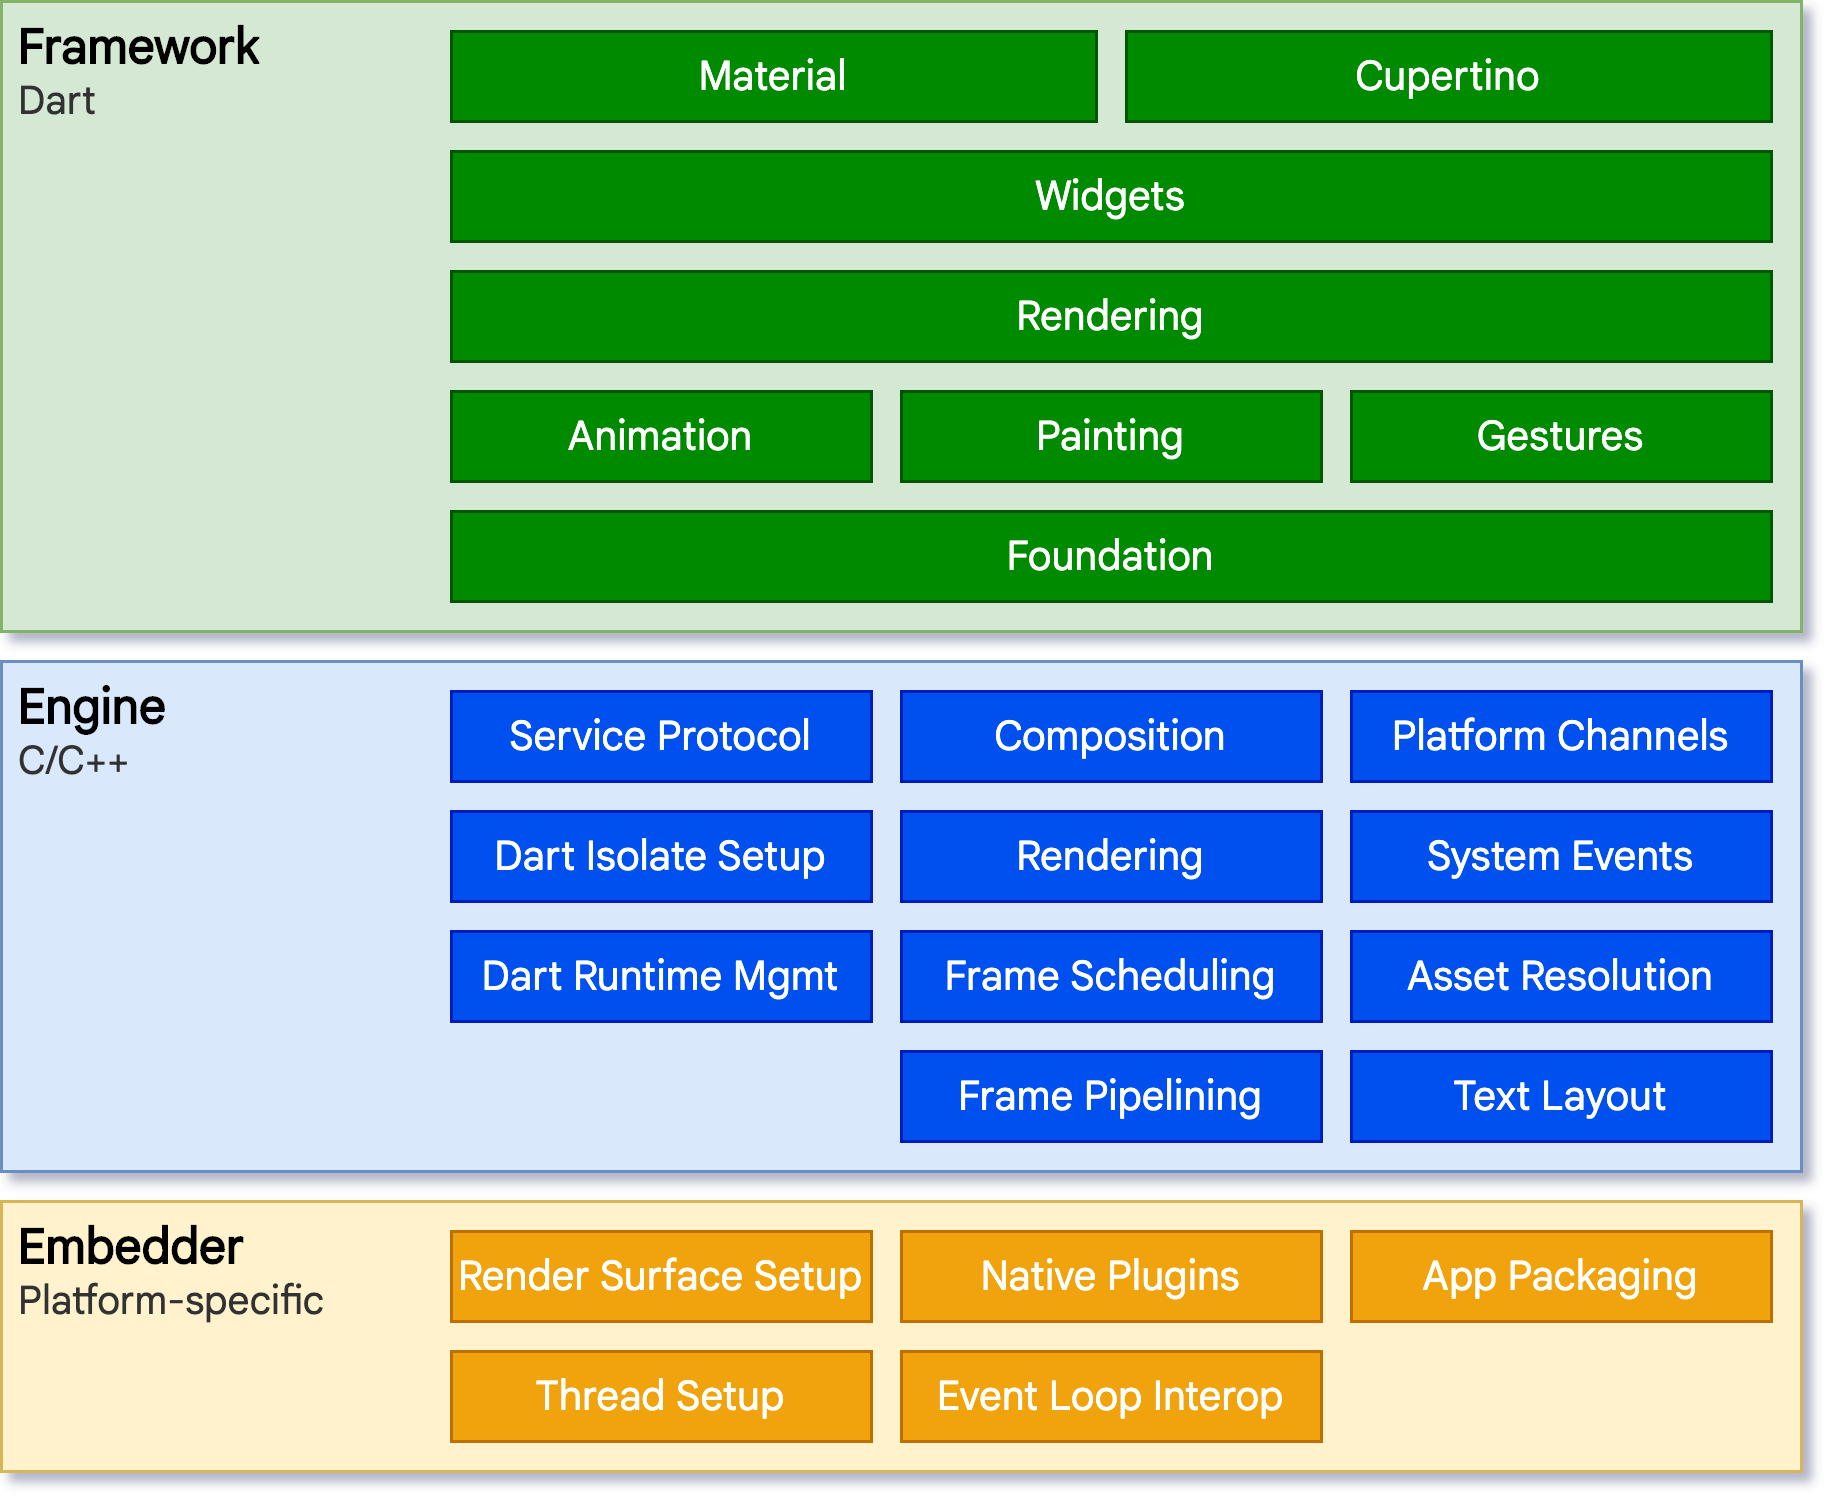
\includegraphics[width=\linewidth]{Image/Flutterarchdiagram.png}
                    \captionof{figure}{Architecture of Flutter\cite{FlutterArch}}
                \end{Figure}

                Another advantage of using Flutter is the adaptability with TensorFlow, since both flutter and TensorFlow are developed by Google, the adaption of TensorFlow to Flutter is easier. Therefore, with using Flutter, the difficulty of model deployment are also reduced.

                In conclusion, we will use flutter SDK as the framework for the multi-platform application development.
            \subsubsection{UI/UX}
                The user interface(UI) and experience(UX) design is another part of the development of the application. In this part, we mainly focus on design of the user interface and experience and the implement of UI/UX.

                A main point in designing UI would be visual effect. Unlike other part in this report, UI design would require work on drawing and designing. There is many professional tools that allows designer to draw out idea user interface. In our platform the main interfaces we need to design are:
                \begin{enumerate}
                    \item Loading page
                    \item Home page
                    \item Camera page
                    \item Survey page
                    \item Information page
                    \item Result page
                    \item Model choosing page
                \end{enumerate}
                Each page should be well-designed with intuitive instruction to users that users can understand the workflow of the application with minimum effort. If necessary, we might need a tutorial teaching the users the correct usage of our application.

                The UX design is similar, the main idea is making all the operations in the platform easily accessible and intuitive. In addition, the wording of instruction and information should be aware of that absolute words need to be avoided. Furthermore, the design of platform should emphasis the information provided in application, especially those generated by NLP is only for reference, seeking for advice from professional dermatologists is still necessary.